

\startappendix{State-Space Model with Kalman Filter}
\label{chapter:appendixA}

%\input chapters/appendix/a1

We adopt the notation from \cite{Petris2008} and modify it for convenience. 


\section{State-Space Model}


The linear Gaussian state-space model is defined in three parts:



\textbf{Observation/measurement equation}


The observations uncertainty $p(y_{t} \mid \mathbf{\alpha}_{t},\theta)$ described by the observation equation

$$y_{t} = F_{t}\alpha_{t}+v_{t},\quad  v_{t}\sim \mathcal NID(0,V_{t}) \, .$$



\textbf{State/transition/process/model equation} 


The process uncertainty of the unknown states $\alpha_{t}$ and their evolution given by the state equations as $p(\alpha_{t} \mid y_{t} \theta)$.  


$$\alpha_{t} = G_{t}\alpha_{t-1}+B_{t} u_{t}+w_{t},\quad  w_{t}\sim \mathcal NID(0,W_{t})\, .$$


\textbf{Parameters to estimated $p(\theta)$ }


$$\theta : { \alpha_t, F_t,  G_t ,V_{t}, W_{t} }\, .$$


\textbf{The initial state distribution }



$$\alpha_{0}\sim \mathcal N(m_0,C_{0})\, ,$$

And then we have:
\textbf{The transition probabilities of state from time $t - 1$ to $t$ }

$$\alpha_t|\alpha_{t-1}   \sim \mathcal N( G_t \, \cdot \alpha_{t-1};W_t) $$

\textbf{The conditional probability of the variable $y$ at time $t$; given that the state of the system, $\alpha$ at time $t$ }

$$y_t|\alpha_t  \sim \mathcal N(F_t \cdot \alpha_t;V_t)$$


where: 


-  $y_{t}$ is the observation of target variable  at time $t$ , with $t = 1,..., T$.



-  $\alpha_t$ is state vector (length $m$), the unobserved / hidden states of the system. In time series setting, $\alpha_t$ will have various components such as trend, seasonality, etc.  







-  $G_t$ is state transition matrix, an $(m \times m)$ matrix, which is applied to the previous state $\alpha_{t-1}$. The unobserved state $x_t$ evolves in time according to the $G_t$ matrix. 







- $F_t$ is the observation model an ( $m \times 1$)  matrix/vector which transforms the true state space into the observed space in our structural time series model. 







- $v_t$ is the measurement errors (observation noise) which are assumed to be zero mean Gaussian white noise with covariance matrix $V_t$. In our structural time series model, it is a scalar/constant ;







- $w_t$ is the state innovations (the process noise) which are assumed to be drawn from a zero mean multivariate normal distribution with covariance matrix $W_t$.







- $B_t$ is the model that predicts what changes based on  control/commands.







- $u_t$ is the control / commands/ input  in time $t$. In our model, we have not included any control or intervention policy, so no $B$ and $u$ terms are in our model. 



- $m_{0}$ is the mean of the initial state; $C_{0}$ is the variance of the initial state.



The initial state, and the noise vectors at each step ${\alpha_0, w_1, ..., w_t, v_1 ... v_t}$ are all assumed to be mutually \textit{independent}.





\section{Kalman Filter} 

The Kalman Filter has two stages: 

\begin{enumerate}
	\item{Predicting the new state and its uncertainty.}
	\item{Correcting with the new measurement.}
\end{enumerate}





\subsection{The state of Kalman Filter}

The state of the filter is represented by two variables:conditional mean(expected value) and covariance.

$$p(\alpha_t \mid y_t) \sim  \mathcal N( m_t, C_{t})$$ 

\begin{enumerate}
	\item{$m_t$, the  posterior state estimate at time $t$ given observations up to  and including those at time $t$;}
	
	
	\item{$C_{t}$, the posterior error covariance matrix (a measure of the estimated accuracy of the state estimate). It reflects the variance of the state distribution.
		
		$$C_{t} = \mathrm{cov}(\alpha_t - m_t)$$
		
					
		}
	
\end{enumerate}




\subsection{Two phases: Predict and Correct} 


We start  with $\theta_0 \sim N(m_0, C_0)$ at time $0$.


\textbf{Predict/(state, error)stage/ (time update)} 


The Predict/time update projects the current state estimate ahead in time. 

$${a}_{t\mid t-1} = \mathbf{G}_{t}{a}_{t-1\mid t-1} + \mathbf{B}_{t} \mathbf{u}_{t}$$



$$\mathbf{R}_{t\mid t-1} = \mathbf{G}_{t} \mathbf{C}_{t-1\mid t-1} \mathbf{G}_{t}^{\text{T}} + \mathbf{W}_{t}$$




where

${a}_{t\mid t-1}$ is one step ahead prediction for (a prior) state.  $B$ and $u$ are control or intervention policies and can be chosen by people to change the state $\alpha$. ${a}_{t\mid t-1}$ is the estimate in next state $\alpha_{t}$; ${m}_{t-1\mid t-1}$ is the estimated state in the last state $\alpha_{t-1}$. The initial state $\alpha_0$ is known.    


$\mathbf{R}_{t\mid t-1}$ is covariance of one step ahead prediction for (a prior) state. $\mathbf{C}_{t-1\mid t-1}$ is the previous error covariance at time $t-1$.  

$\mathbf{W}$: the covariance matrix of the error noise.

Then we have:

$$\alpha_t|y^{t-1} \sim N(a_t, R_t)$$

where $y^{t-1}$ is \{${y_0, y_1, y_2,..., y_t,...}$\} up to time $t-1$. 

We also can get one step ahead prediction for the observation $f_t$: 

$$f_t = F_t \cdot a_t$$

$$Q_t = F_t R_{t-1} F_t^\prime + V_t$$

And we have 

$$y_t|y^{t-1} \sim N(f_t, Q_t)$$

\textbf{Correct /Update stage/  measurement update}

The Correct/measurement update adjusts the projected estimate by an actual measurement at that time.


\textit{Updated (a posteriori) state estimate $m_{t\mid t}$} with new observation $y_t$. $m_{t\mid t}$ is a weighted average of latest estimate and gain from observation. 


$$m_{t\mid t} = a_{t\mid t-1} + \mathbf{K}_t \tilde{v}_t$$  


\textit{Updated (a posteriori) estimate covariance $\mathbf{C}_{t|t}$} 



$$\mathbf{C}_{t|t} = (I - \mathbf{K}_t \mathbf{F}_t) \mathbf{R}_{t|t-1}$$


Then we have posterior of state at time $t$:

$$\alpha_t|y^t \sim N(m_t, C_t)$$


Where $\tilde{v}_t$  is \textbf{prediction error}, and $K$ is \textbf{Optimal Kalman gain}. 

When the \textbf{prediction error}  $\tilde{v}_t$  is non-zero, there is new information about the system, so the state  $\alpha$ should be modified. $\tilde{v}_t$ is also called Measurement innovation or the predictive residual.  

The prediction error $\tilde{v}_t$ reflects the discrepancy between the predicted measurement $E(y_{t\mid t-1})$ and the actual measurement $y_t$. In our case, the prediction error is a scalar $\tilde{v}_t$:

  
$$\begin{aligned}
\tilde v_t  &= y_t -E(y_{t\mid t-1} ) \\
& = y_t - F_{t} E(\alpha_{t\mid t-1} ) \\
& = y_t -f_{t}
\, ,
\end{aligned}$$

and the covariance matrix of $\tilde{v}_t$ is  

$$\mathbf{S}_{t} = \mathrm{cov}(\tilde{v}_t) 
 = \mathbf{F}_t \mathbf{R}_{t\mid t-1} \mathbf{F}_{t}^\text{T} + \mathbf{V}_t \, ,$$

where $V_t$ describes the noise in the observation $\mathbf{y}_t$.


The contribution of $\tilde{v}_t$ to the state vector is weighted by the \textbf{Optimal Kalman gain} $\mathbf{K}_t$. $\mathbf{K}_t$ measures how much to trust a new observation ${y}_t$. It can be a matrix, and in our case it is a vector.



An \textbf{Optimal Kalman gain} $\mathbf{K}_t$ is chosen to be the gain or blending factor so that we minimize the a posterior estimation error covariance  $\mathbf{C}$:


$$\mathbf{K}_t = \mathbf{R}_{t\mid t-1}\mathbf{F}_t^T \mathbf{S}_t^{-1}$$



where $\mathbf{S}_t$ is prediction error covariance.  $\mathbf{F}_t$ describes  how the observation reflects the state in the model (a function of how much influence goes from observation to state vector).


\subsection{Optimal Kalman gain} 


The Kalman filter is a minimum mean-square error estimator. The error in the  posterior state estimation is


$$\alpha_{t} - m_{t\mid t} \, .$$



We seek to minimize the expected value of the square of the magnitude of this vector, $\textrm{E}[\|\alpha_{t} - m_{t|t}\|^2]$. This is equivalent to minimizing the trace of the a posteriori estimate of the covariance matrix $\mathbf{C}_{t|t}$ . Solving this optimization problem for $\mathbf{C}_{t|t}$ yields the optimal Kalman gain  $\mathbf{K}_t$:


$$\mathbf{K}_t \mathbf{S}_t = (\mathbf{F}_t \mathbf{R}_{t\mid t-1})^\text{T} = \mathbf{R}_{t\mid t-1} \mathbf{F}_k^\text{T}$$


$$\mathbf{K}_{t} = \mathbf{R}_{t\mid t-1} \mathbf{F}_t^\text{T} \mathbf{S}_t^{-1} \, .$$


This gain  is  the optimal Kalman gain and yields MMSE (minimum mean square error ) estimates.  






\startappendix{Data of Predictors}
\label{chapter:appendixB}

Predictors are all seasonally adjusted, detrended, and scaled. They are all stationary, as determined by  the ADF and KPSS tests, at the 5\% significance level. 


\section{Unemployment rate: Monthly, 1980/07-2015/03}  


The unemployment rate data is monthly seasonally adjusted data which covers all aged 15 and over in the labor force in Canada. The data is taken from St. Louis Fed. website. The data has been detrended, deseasonalized and scaled, and then it is skipping sampled as was described in section 3.2.2. 

\begin{figure}[h]
	\centering
	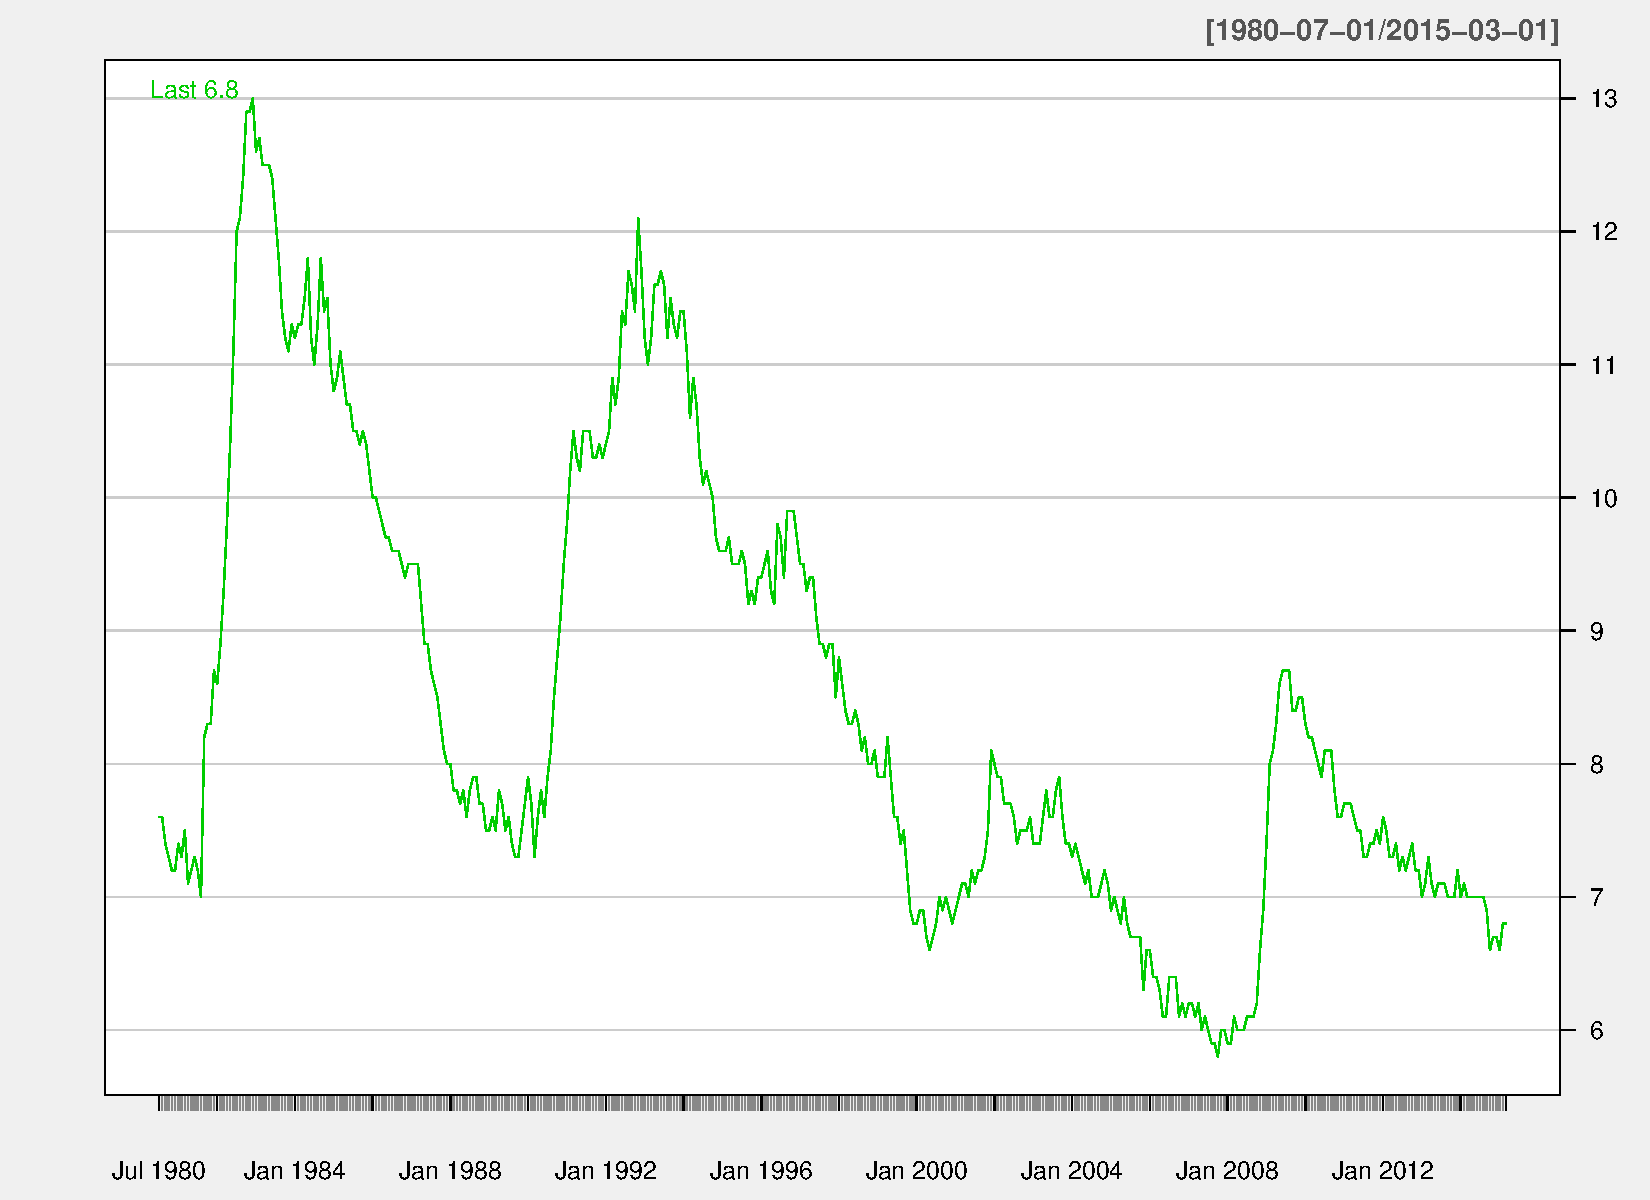
\includegraphics[width=0.7\linewidth]{Figures/labor-report}
	\caption{Unemployment Rate for Canada}
	\label{fig:labor-report}
\end{figure}


\section{Spread between 3 months treasury bills yields and 10 year's government bond yields. Monthly, 1980/07 - 2015/03} 



The spread is calculated by subtracting interest rates of 3 month treasury bills for Canada from interest rate of 10 year's government bond for Canada. Both data is taken from St Louis Fed website.


It is detrended, deseasonalized and scaled. And then it is skipping sampled  was described in section 3.2.2. 


\begin{figure}
	\centering
	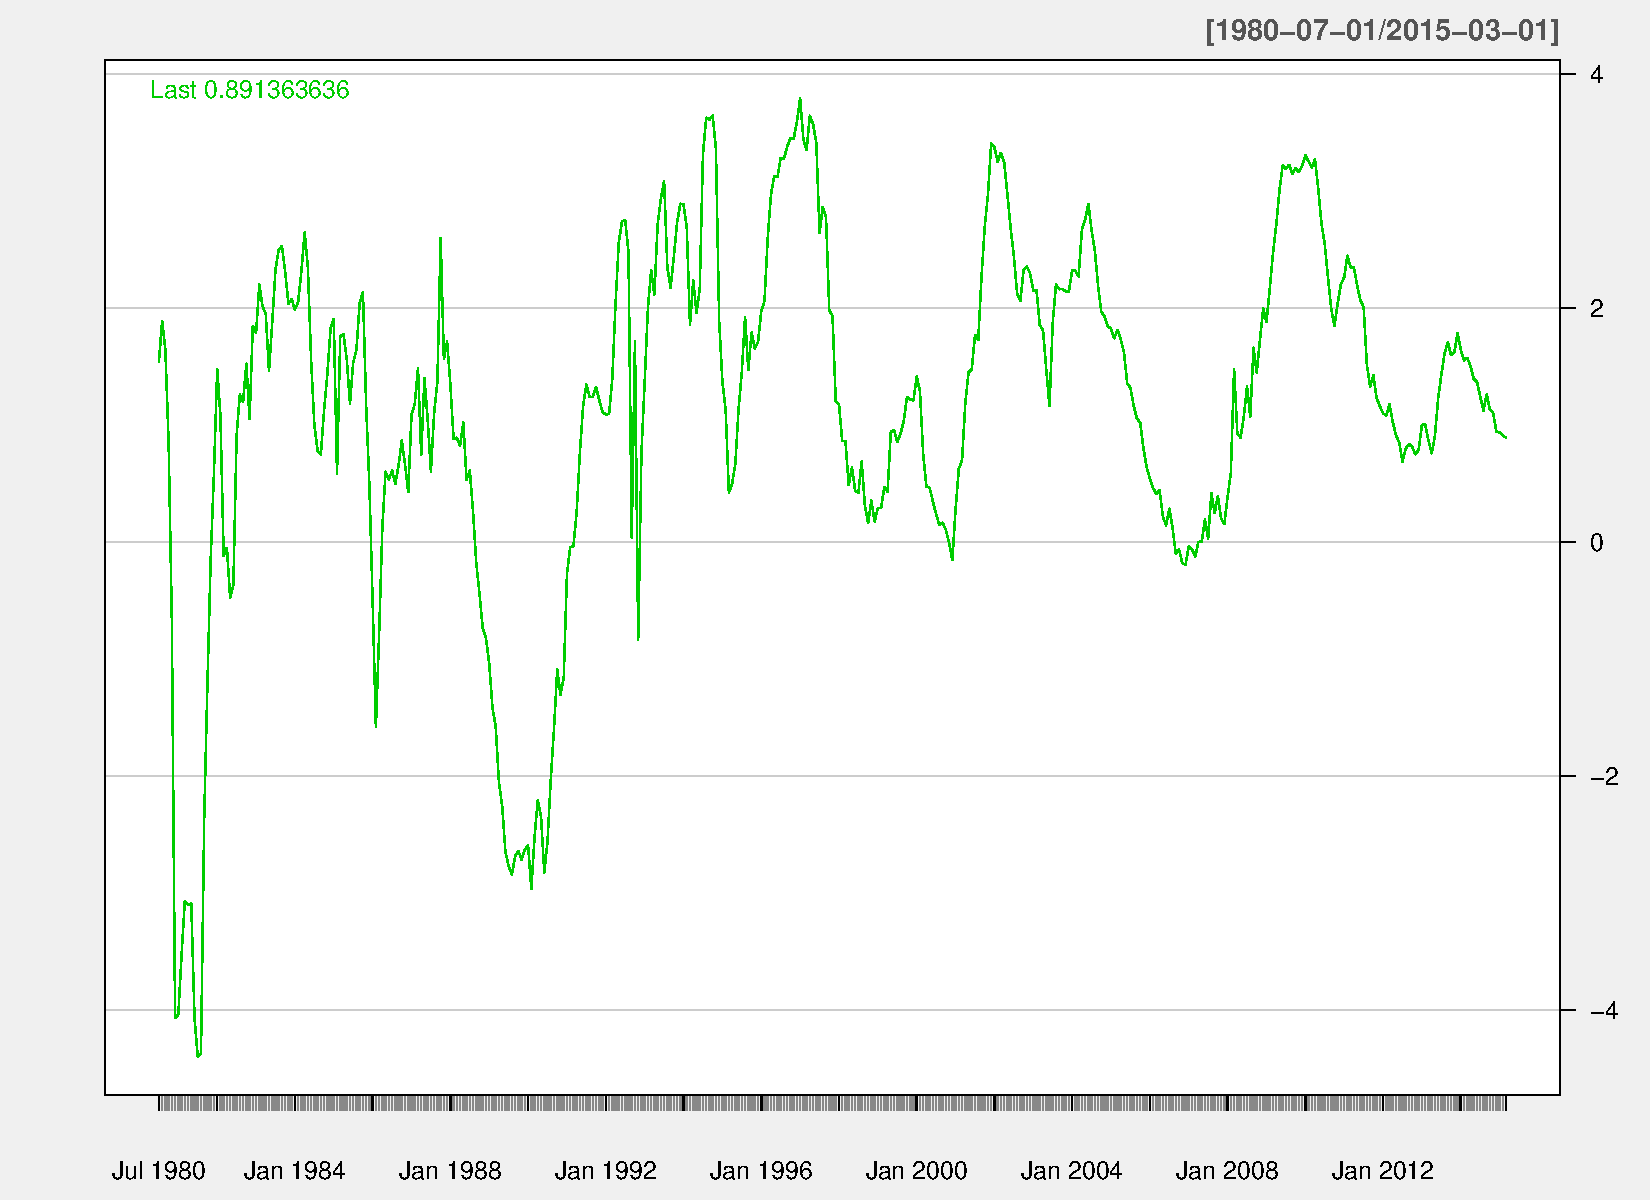
\includegraphics[width=0.7\linewidth]{Figures/spread-report}
	\caption{Spread between 3 month and 10 year government bond interest rate}
	\label{fig:spread-report}
\end{figure}



\section{Toronto Stock Exchange (S\&P/TSX) Composite index 1980/07/01-2015/05/28}


S\&P/TSX Composite index is daily and is taken from St. Louis Fed website.

Before included in our model, it is transformed to log difference and is detrended, deseasonalized and scaled to achieve stationary. 

In order to match up the quarterly target variable, it is skipping sampled  was described in section 3.2.2. 

\begin{figure}[h]
\centering
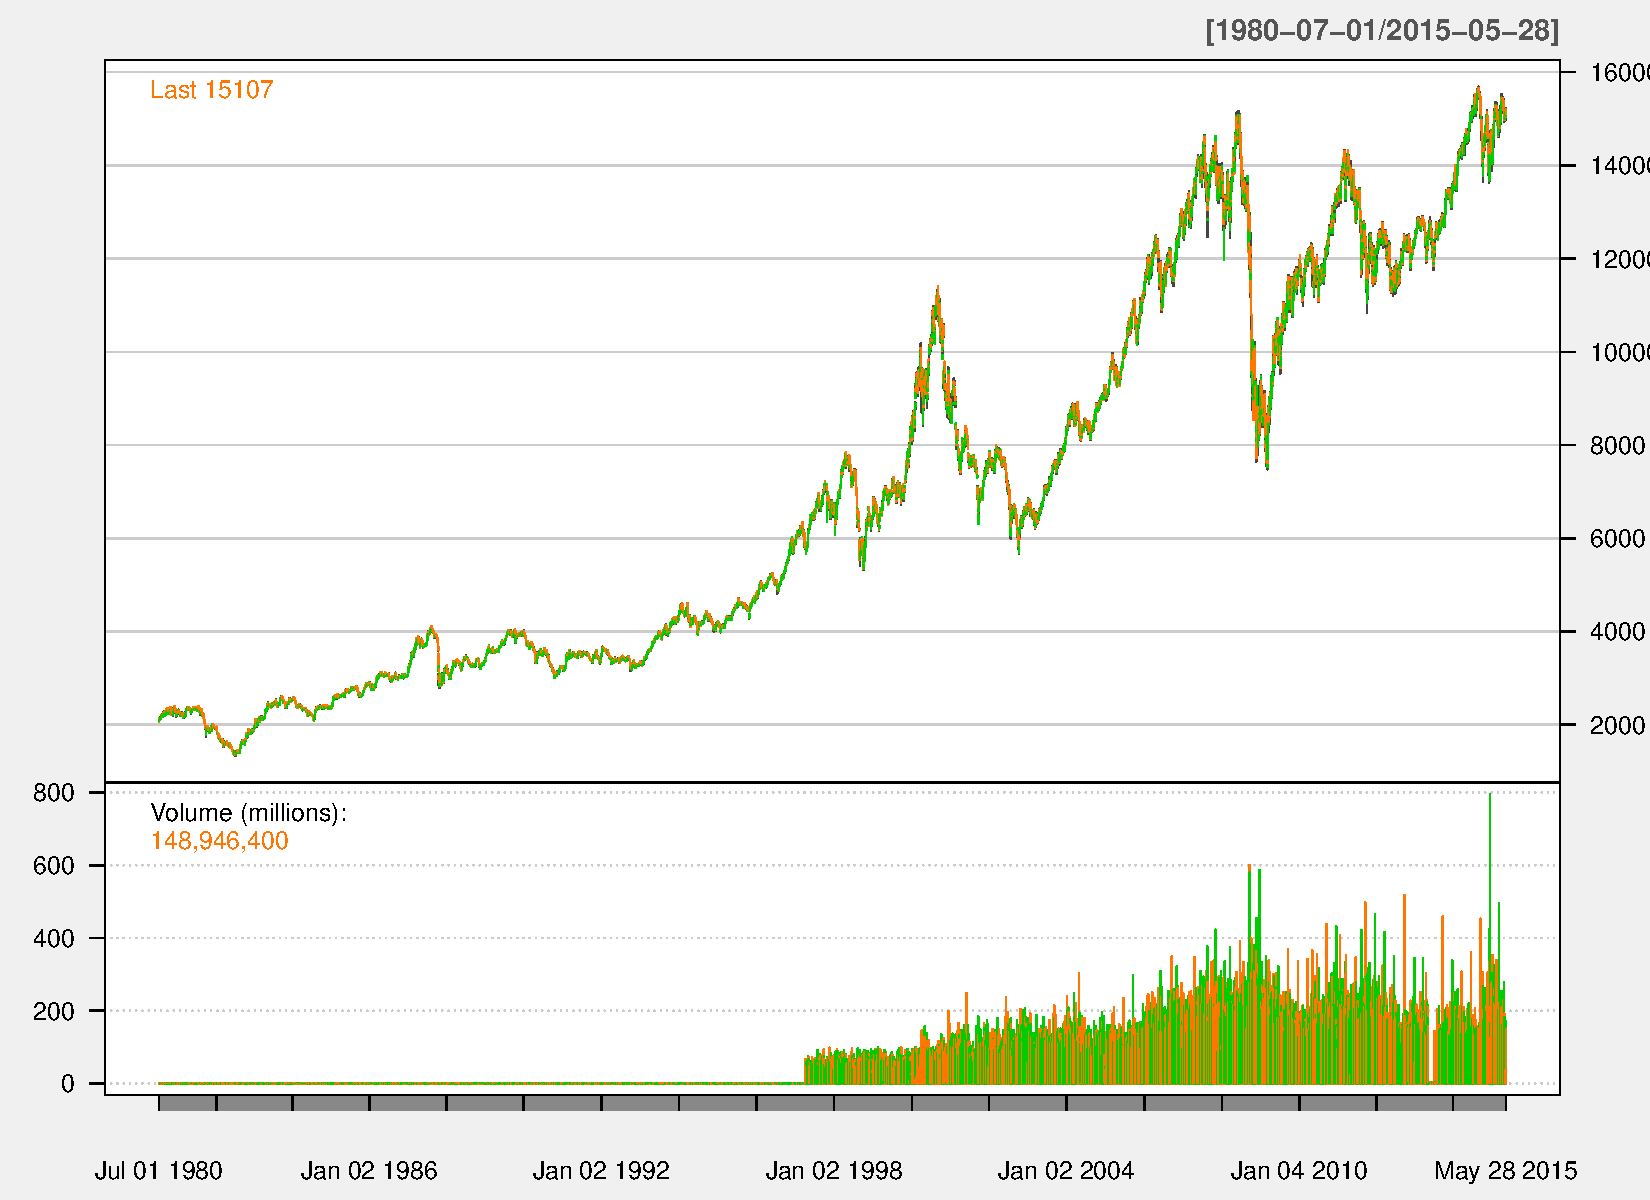
\includegraphics[width=0.7\linewidth]{Figures/tsx-report}
\caption{TSX stock market index}
\label{fig:tsx-report}
\end{figure}


\section{Housing starts, monthly, 1980/07-2015/03} 

The housing starts data is from Canada Mortgage and Housing Corporation. It covers housing under construction and completions in centres with 10,000 and over population in selected census metropolitan areas. 

The data is detrended, deseasonalized and scaled, and then it is skipping sampled  was described in section 3.2.2. 

\begin{figure}
\centering
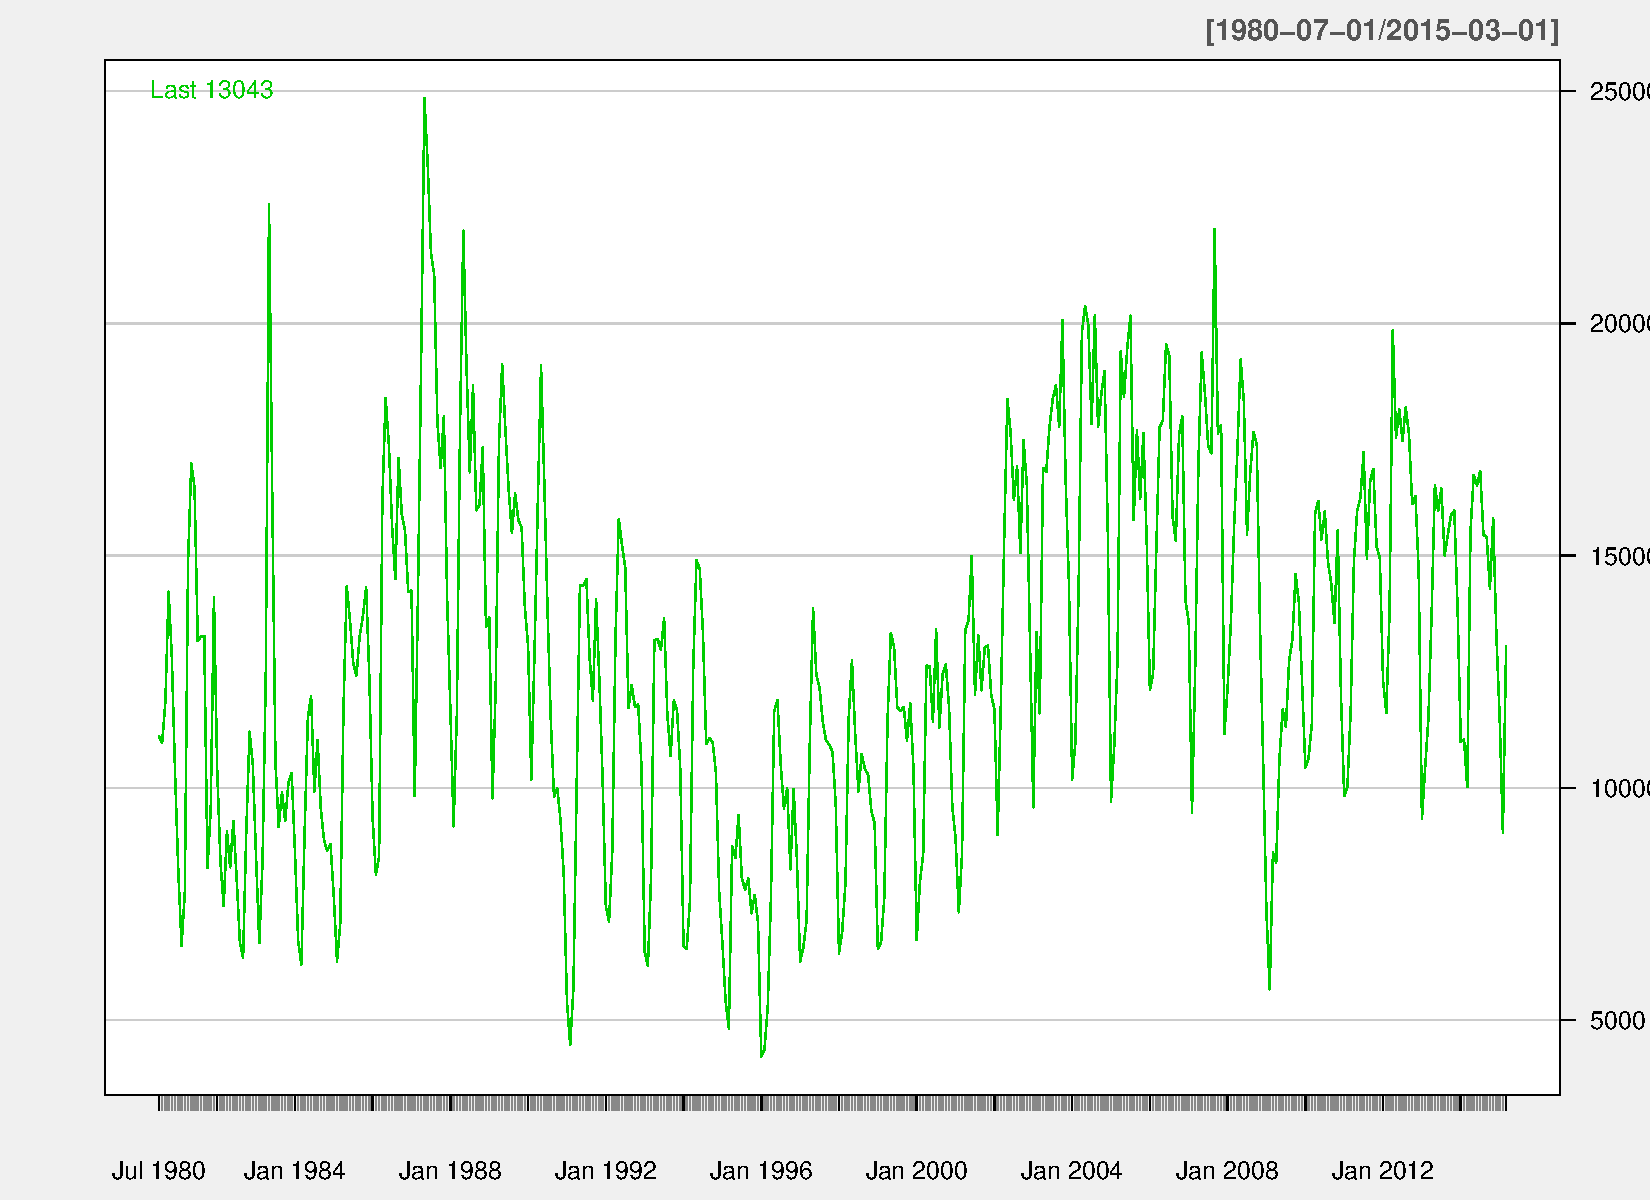
\includegraphics[width=0.7\linewidth]{Figures/house-report}
\caption{Housing starts}
\label{fig:house-report}
\end{figure}


\section{Crude Oil Price: West Texas Intermediate (WTI), daily, 1980/07/01-2015/05/28} 

The oil price data  is daily and is taken from St 
Louis Fed website.

Before included in our model, it is transformed to log difference and is detrended, deseasonalized and scaled to achieve stationary. 

In order to match up the quarterly target variable, it is skipping sampled  was described in section 3.2.2. 

\begin{figure}
	\centering
	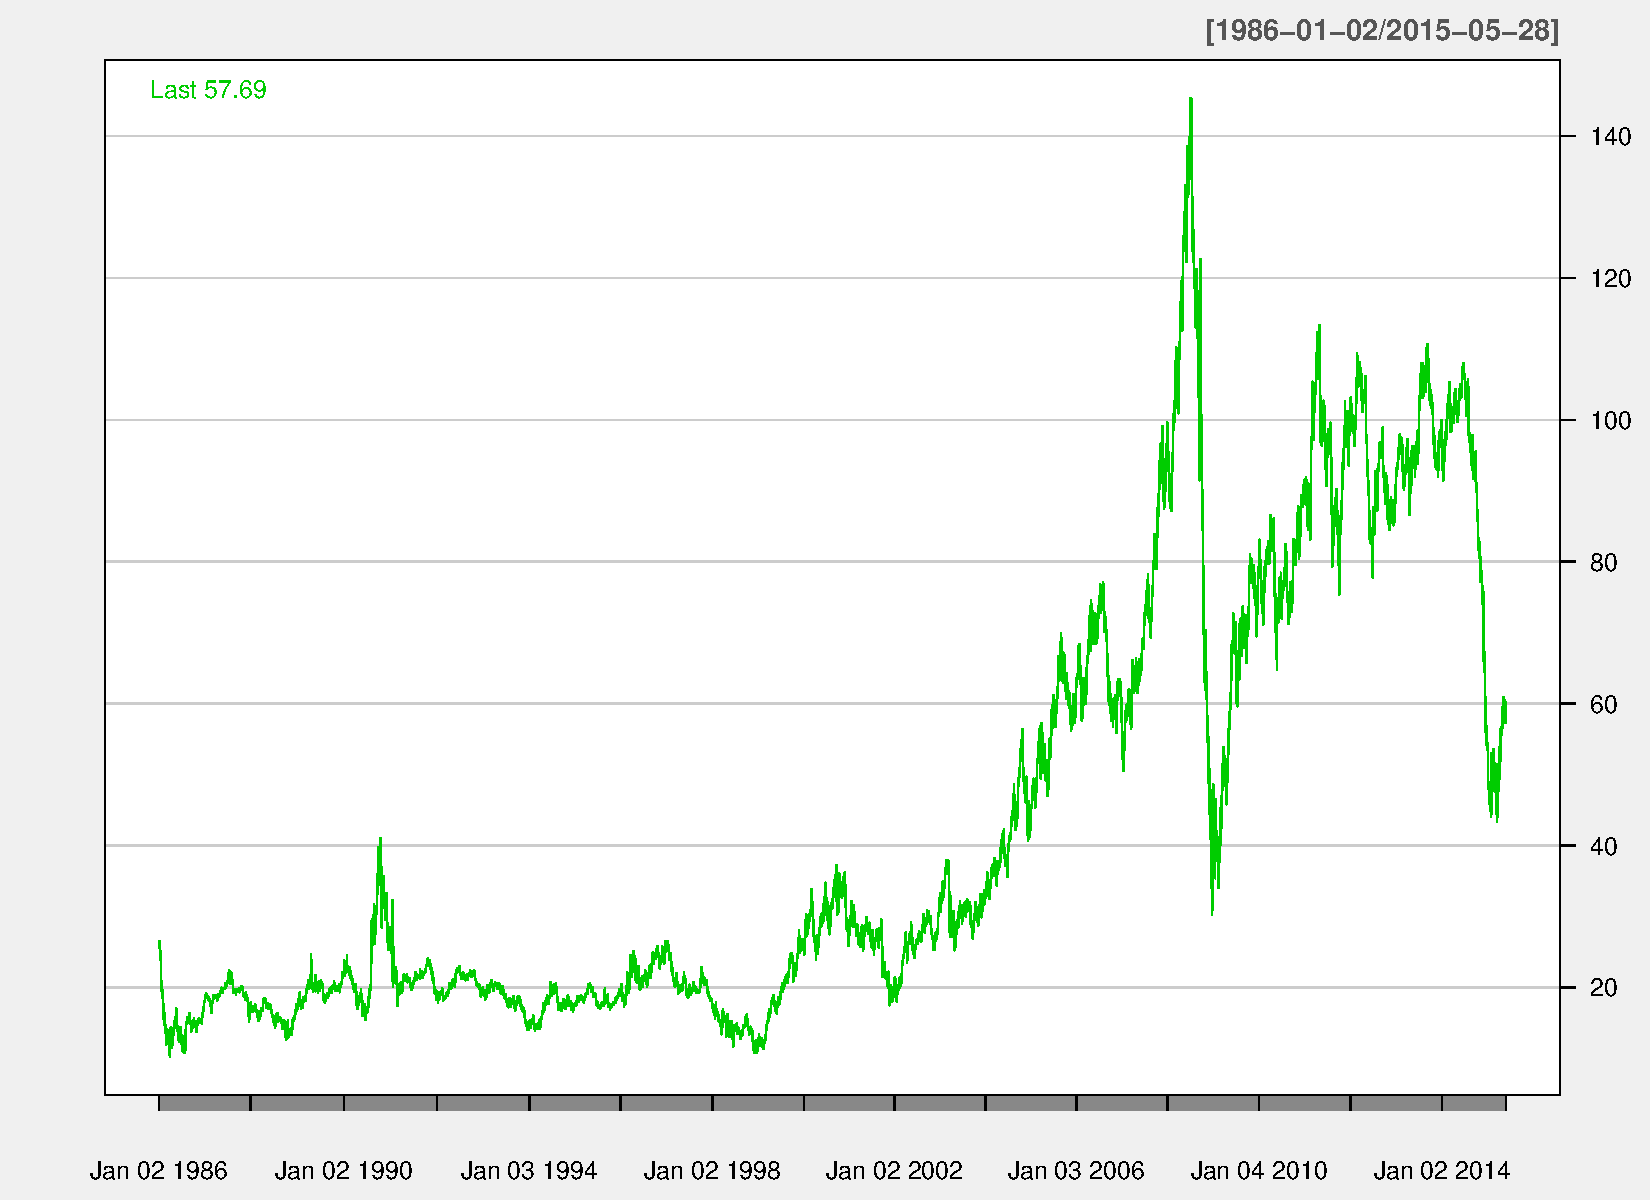
\includegraphics[width=0.7\linewidth]{Figures/oil-report}
	\caption{Crude Oil Price}
	\label{fig:Oil Price}
\end{figure}


\startappendix{Model Specification}
\label{chapter:appendixC}


\section{Generalized local trend model with regression}


The generalized local linear trend model is more complicated than a regular local trend model. In our practice, we also add a ar(t) term in the equation.



\textbf{Observation equation} (level + regression): 



$$y_t = \mu_t + c_t + z_t + v_{t}, \quad v_{t} \sim N(0, V) \, .$$



It assumes the level moves according to a random walk, but the slope moves according to an AR(1) process centered on some potentially nonzero value $D$. The equation for the mean is


\textbf{State equation 1} (random walk + trend ):  



$$\mu_{t+1} = \mu_{t} + b_{t} +  w_{1t}, \quad w_{1t} \sim N(0, W_{1}) \, .$$



The equation for the slope $b$  is



\textbf{State equation} 2 (AR(1) for trend):  



$$b_{t+1} = D + \phi  (b_t - D) + w_{2t}, \quad w_{2t} \sim N(0, W_{2}) \, .$$



The prior distribution for this model has four independent components. There is an inverse gamma prior on the level standard deviation, sigma.level; an inverse gamma prior on the slope standard deviation sigma.slope; a Gaussian prior on the long run slope parameter $D$; and a potentially truncated Gaussian prior on the AR(1) coefficient $\phi$. 

The slope exhibits short term stationary variation around the long run slope $D$ when absolute value of the prior on  $\phi$ is less than 1  \cite{Scott2015}. The parameter  $\phi$ represents the learning rate at which the local trend is updated. Hence, the model balances short-term information $(b_t - D)$  with information $D$ from the distant past.


\textbf{State equation} 3 (dynamics of ar(4) process):  


$$c_t = \psi_1 c_{t-1} + \psi_2 c_{t-2} +\psi_3 c_{t-3} +\psi_4 c_{t-4}, \quad w_{3t} \sim N(0, W_{3}) \, .$$

\textbf{Regression component}: $$z_t = \beta x_t$$ 
we can append a constant $1$ of the state vector $\alpha$ and append $z_t$ to observation matrix $F$. By doing so, we only increase the dimension of state vector $\alpha$ by one. 






\section{ARIMA model}
\label{sec:arima}

We use  Hyndman's ``forecast" package in R to fit ARIMA models and estimate one step ahead forecast \cite{Hyndman2015}. The ARIMA models are chosen according to either AIC, AICc or BIC value in the ``auto.arima" function in ``forecast" package. In the test period 2003 to 2015, there are 48 models. The first 35 models selected by ``auto.arima" are AR(1) with an intercept. The last 13 models are AR(2) with an intercept. 

% Please add the following required packages to your document preamble:
% \usepackage{booktabs}
\begin{table}[ht]
	\centering
	\begin{tabular}{@{}llll@{}}
		\toprule
		Year/Quarter & AR1     & AR2     & Intercept       \\ \midrule
		2003/02    & 0.55&  & 0.658  \\
		2003/03    & 0.556 &  & 0.638   \\ 
		2003/04    & 0.552 &  & 0.643  \\
		2004/01    & 0.552 &  & 0.643  \\
		2004/02    & 0.549 &  & 0.650  \\
		2004/03    & 0.548 & & 0.666  \\
		2004/04    & 0.552 & & 0.673  \\
		2005/01    & 0.552 & & 0.673  \\
		.\\
		.\\
		.\\
		2013/02    & 0.580 & -0.052 &  0.593 \\
		2013/03    & 0.576 & -0.047 &  0.589 \\
		2013/04    & 0.575 & -0.046 &  0.591  \\
		2014/01    & 0.576 & -0.046 &  0.593 \\
		2014/02    & 0.575 & -0.046 &  0.585 \\
		2014/03    & 0.569 & -0.041 &  0.594 \\
		2014/04    & 0.569 & -0.042 &  0.595 \\
		2015/01    & 0.569 & -0.043 &  0.592 \\
		 \bottomrule
	\end{tabular}
	\caption{ARIMA models 2003-2015}
	\label{ARIMAmodels}
\end{table}


Table ~\ref{ARIMAmodels} shows that the fitted models chosen by ``auto.arima" function do not change much when the we move forward during the test period 2003 to 2015. Since an ARIMA model is univariate model, one extra data point usually does not provide much information for refitting a model.




  

\section{Boosting model}
\label{sec:boost}
We fit the Boosting model by using the ``GBM" package in R \cite{Ridgeway2015}. In the Boosting model, we also include the AR terms of target variables up to 7 th lag. For a Boosting model, there are many hyper-parameters for tuning. We choose the number of trees in the model as 400, which decides how many iterations we do in the model. We choose 0.01 as the shrinkage parameter, which a regularization parameter to determine how fast the algorithm moves across the gradient. Decreasing shrinkage usually improves performance, but requires more trees for the ensemble. We choose 20 as the depth of the model, which means each tree will evaluate 20 decisions, and each decision will yield 20 nodes from the  prior node. We choose 5 as the minimum number of observations in the terminal node.   

\section{Prior distributions and prior elicitation}
\label{sec:prior}


Given $\gamma$,  the prior for the precision follows a Gamma distribution with parameters $\frac{df}{2}$ and $\frac{ss}{2}$. Thus, the reciprocal of the mean of the Gamma distribution $ss/df$ is a prior estimate of $\sigma^2$. 


To elicit priors for $ss$ and $df$, it could be done by using a device $ss = df (1-R^2) s_{y^*}^2$. $R^2$ is expected $R^2$, and $s_{y^*}^2$ is the sample variance of the modified target variable, which is $s_{y^*}^2 = \sum_{t=1}^{T} \frac{({y^*}_t - \bar{y^*})^2}{T-1}$.  

The ``Slab" prior is a very weakly informative prior which is close to being flat. In some sense,  $ss$ can be interpreted as a prior sum of squared error, and the $df$ can be interpreted as a prior sample size. (which decides the weight given to the guess at $R^2$)

Using our previous knowledge of parameters, we can set our values for the parameters $\pi$, $b_{\gamma}$, $\Omega^{-1}$, $df$, and $ss$. For  simplicity, we also can just specify an expected model size $n$, $\kappa$, and expected $R^2$, and a sample size $df$. In our case, we use the default values $R^2 = 0.5$ and $df = 0.01$ in the R package ``bsts" \cite{Scott2015}. 
We set ``expected model size" to $4$, so the $\pi = 4/602$ is the average probability to included in the model.

For elicitation of the prior of $\Omega^{-1}$, we have $\Omega^{-1} \propto X^T X$, but  it is not feasible when $X^T X$ is singular or not full rank, which is possible in our design matrix. 


First, we have a fat regression, the number of predictors is larger than the number of observation. Second, we have many macroeconomic variables as predictors that are closely correlated. There are possible strong multi-collinearity in design matrix. When $X^T X$ is rank deficient, $p(\beta, \sigma | \gamma)$ is improper for some value of $\gamma$. \citeA{Scott2014b} propose that we can averaging $X^T X$ by its diagonal to restore propriety.

$$\Omega^{-1} = \frac{\kappa}{T}  [ w X^T X +(1-w)  diag(X^T X) ] .$$

In their research, \citeA{Brodersen2014} set  $\kappa = 1$ and $w = 1/2$ as default values.  The matrix $X^T X / \sigma^2$ is the total Fisher information matrix in the full data,  and $ \frac{1}{T}  X^T X$  is the average information in a single observation. 


\section{Estimating the model using Markov Chain Monte Carlo}
\label{sec:mcmc}

We follow \citeA{Scott2014b} in that we draw samples using Markov Chain Monte Carlo. 

Say $y$ is the target series, $\alpha$ is vector of the states, and $\theta$ is vector of the parameters. The complete data posterior distribution is 

$$p(\theta , \alpha| y)  \propto p(\theta_0) p(\alpha_0) \prod_{t=1}^{T} p(y_t | \alpha_t , \theta) p(\alpha_t | \alpha_{t-1}, \theta).$$

We can use Gibbs sampling to draw $p(\alpha | \theta, y)$ and $p(\theta | \alpha, y)$ alternatively. And we can get  a sequence of samples from a Markov chain with stationary distribution $p(\theta , \alpha| y)$. This chain consists of $(\theta, \alpha)_0$,$(\theta, \alpha)_1$ , $...$ a sequence of samples.   


Since $\alpha$ is a Markov Chain, the time series components and regression components are independent conditional on $\alpha$. Let $\psi$ is vector of the parameters associated with $\alpha$.  $\theta$ includes $\beta, \sigma^{-2}$, and $\psi$. The $p(\theta | \alpha, y)$ can be decomposed into several independent conditional posterior distribution of the $\alpha$. Then we have

$$p(\psi, \theta, \sigma^{-2}|\alpha, y ) = P(\psi |\alpha, y) p(\theta, \sigma^{-2} |\alpha, y) $$

\subsection{Sampling $\psi$}

Suppose we have a local linear trend model with two states. 


\begin{itemize}
	\item {State equation 1 (random walk + trend): $$\mu_t = \mu_{t-1} + b_{t-1} + w_{1t}, \quad w_{1t} \sim N(0, W_{1})$$}
	
	\item {State equation 2 (random walk for trend): $$b_t = b_{t-1} + w_{2t}, \quad w_{2t} \sim N(0, W_{2})$$}
\end{itemize}








Assume independent Gamma priors for state variances:
 $$\frac{1}{W_{1}}  \sim \Gamma(df_1/2, ss_1/2),$$  
 $$\frac{1}{W_{2}}  \sim \Gamma(df_2/2, ss_2/2),$$
 
In the Gamma distribution, the reciprocal of the expectation $ss/df$ is a prior estimate of $W$, and $df/ss$ is a prior estimate of precision $1/W$. The prior parameter $ss$ can be interpreted as a prior sum of squared error, and $df$ is the weight assigned to the prior estimate of precision $1/W$. 

If we do not have enough information about the prior distribution of the state variance $W$, we can choose a small value for $df$ and small value for $df/ss$. \citeA{Brodersen2014} choose $1/W \sim \Gamma (10^{-2}, 10^{-2} s_y^2)$ as their default priors for a seasonal and local linear trend model, where $s_y^2 = \sum_{t}^{T} \frac{(y_t - \bar{y})^2}{(T-1)}$ is the sample variance of the target variable. In this way, they scaling the sample variance to elicit a prior for $W$. Scaling by the sample variance is similar to scaling  the data before the analysis. By scaling in the prior,  they can model the data on its original scale \cite{Scott2014a,Brodersen2014}.  
 
 
The full conditional posterior distribution is the product of two independent Gamma distributions:

$$p(1/W_{1}, 1/W_{2}|\alpha) = \Gamma ( \frac{df_1 + T -1}{2}, \frac{SS_1}{2} ) \Gamma ( \frac{df_2 + T -1}{2}, \frac{SS_2}{2} ) ,$$ 

where $$SS_1 = ss_1 + \sum_{t=2}^{T}(\mu_t - \mu_{t-1} - b_{t-1})^2$$

$$SS_2 = ss_2 + \sum_{t=2}^{T}(b_t - b_{t-1})^2$$

Given the $\alpha: \mu, b$, we can draw $W_{1}$ and $W_{2}$ from their full conditional distributions. 


\subsection{Sampling $\theta, \sigma$}

The full distribution for $\theta, \sigma$ is independent conditional on $\alpha$. 
 
Suppose observation equation is: 
 $$y_t = \mu_t + \beta \mathbf{x}_t + v_{t}, \quad v_{t} \sim N(0, V)$$  
 
  
 
We subtract the target time series component $\mu_t$ from $y_t$, and get an axillary variable $y^* = y_t - \mu_t$.  Then we have  
 
 
$$y_t^* = y_t - \mu_t = \beta x_t + \epsilon_t \sim N(\beta x_t, \sigma^2)$$
 


And we are left with a standard spike-and-slab regression.  $\sigma^{2}$ is the overall variance level. We can use ``stochastic search variable selection"(SSVS) algorithm to draw from $p(\beta_{\gamma}, \sigma^2 | \gamma, \alpha, \mathbf{y}^*)$, where vector $\mathbf{y}^* = y_{1:T}^*$ is all the information about $y^*$ up to time $T$.   
 
 
A ``slab" prior includes:


$$ p(\beta, \sigma^{-2},\gamma) = p(\beta \mid \gamma, \sigma^{-2})p(\sigma^{-2} \mid \gamma )p(\gamma)  \,  ,$$
  
 $$ \beta_{\gamma} \mid \sigma^{2} ,\gamma  \sim N(b_{\gamma}, \sigma^{2}(\Omega_{\gamma}^{-1})^{-1}) \,  ,$$
 
 
 $$\frac {1}{\sigma^{2}} \mid \gamma \sim  \Gamma(\frac{df}{2}, \frac{ss}{2})  \,  ,$$
 
 
Then conditional on $\gamma$, the joint posterior distribution for $\beta$ and $\sigma^2$ can be estimated from standard conjugacy formula \cite{Gelman2013} :   
 
 
 
 
 
 $$\beta_{\gamma} \mid \sigma, \gamma, \mathbf{y}^*, \alpha  \sim  N(\tilde{\beta_{\gamma}}, \sigma^2(V_{\gamma}^{-1})),$$  
 
 
 
 
 $$\frac {1}{\sigma^{2}} \mid \gamma, \mathbf{y}^*, \alpha \sim  \Gamma(\frac{df+T}{2}, \frac{ss + \tilde{S}}{2}),$$  
 
where $$V_{\gamma}^{-1} = X_{\gamma}^T X_{\gamma} + \Omega_{\gamma}^{-1},$$ 
 
 $$ \tilde{\beta_{\gamma}} =  (V_{\gamma}^{-1})^{-1} (X_{\gamma}^T y_{\gamma}^* + \Omega_{\gamma}^{-1} b_{\gamma}),$$
 
 $$\tilde{S} = \sum_{t=1}^{T} (y_{\gamma}^* - \mathbf{x}^T \tilde{\beta_{\gamma}})^2 +   (\tilde{\beta_{\gamma}}- b_{\gamma})^T \Omega_{\gamma}^{-1} (\tilde{\beta_{\gamma}}- b_{\gamma}) = y_{\gamma}^{*T} y_{\gamma}^* + b_{\gamma}^T \Omega_{\gamma}^{-1} b_{\gamma} - \tilde{\beta_{\gamma}}^T V_{\gamma}^{-1} \tilde{\beta_{\gamma}},$$ 
 
\subsection{Sampling $\gamma$} 
 
The prior distribution for $p(\gamma |  \mathbf{y}^*, \alpha)$ is :



$$p(\gamma \mid \mathbf{y}^*, \alpha) \propto \frac{|\Omega^{-1}|^{1/2}}{|V_{\gamma}^{-1}|^{1/2}} \tilde S^{-\frac{df+T}{2}}  \, ,$$

Under Zellner's g-prior, 


 $$\frac{|\Omega^{-1}|}{|V_{\gamma}^{-1}|} = \left(\frac{\kappa/T}{1+ \kappa/T}\right)^{|\gamma|}$$
 
where $|\gamma|$ is the number of the included predictors. In general,  $|\Omega^{-1}| \le |V_{\gamma}^{-1}|$. This implies that $p(\gamma |  \mathbf{y}^*, \alpha)$ is tends to pick models with few predictors and small residual variation. 



Due to the conjugacy, we can get analytical expression for the marginal posterior of $\gamma$ by marginalizing over  $\beta_{\gamma}$ and ${1}/{\sigma^{2}}$:



$$\gamma \mid \mathbf{y}^*, \alpha \sim C(\mathbf{y}^*) \frac{|\Omega^{-1}|^{1/2}}{|V_{\gamma}^{-1}|^{1/2}} \frac{p(\gamma)}{(ss + \tilde{S})^{\frac{T}{2} -1}} \, ,$$

where $C(\mathbf{y}^*)$ is a normalizing constant. 

We can use a Gibbs sampling to draw $\gamma_i$ given $\gamma_{-i}$ and $p(\gamma |  \mathbf{y}^*, \alpha)$. $\gamma_{-i}$ is other $\gamma_{j}$ in $\gamma$ where $j \neq i$.



Since the calculation of $p(\gamma |  \mathbf{y}^*, \alpha)$ only need to compute those matrices associated with $\gamma = 1$,  the SSVS is tractable when computating a system with many predictors \cite{Scott2014b}.
 